\section{Spring framework}

\begin{definition}[\textit{Framework}]
    A software framework is an integrated collection of components, set of applications, conventions, principles and common practices for design and development of software
\end{definition}
Spring stands out as one of the most widely embraced Java-based frameworks for constructing distributed software systems. 
This framework adeptly manages the underlying infrastructure, enabling developers to concentrate on crafting application logic. 
Its robust support from the community adds to its popularity.
\begin{figure}[H]
    \centering
    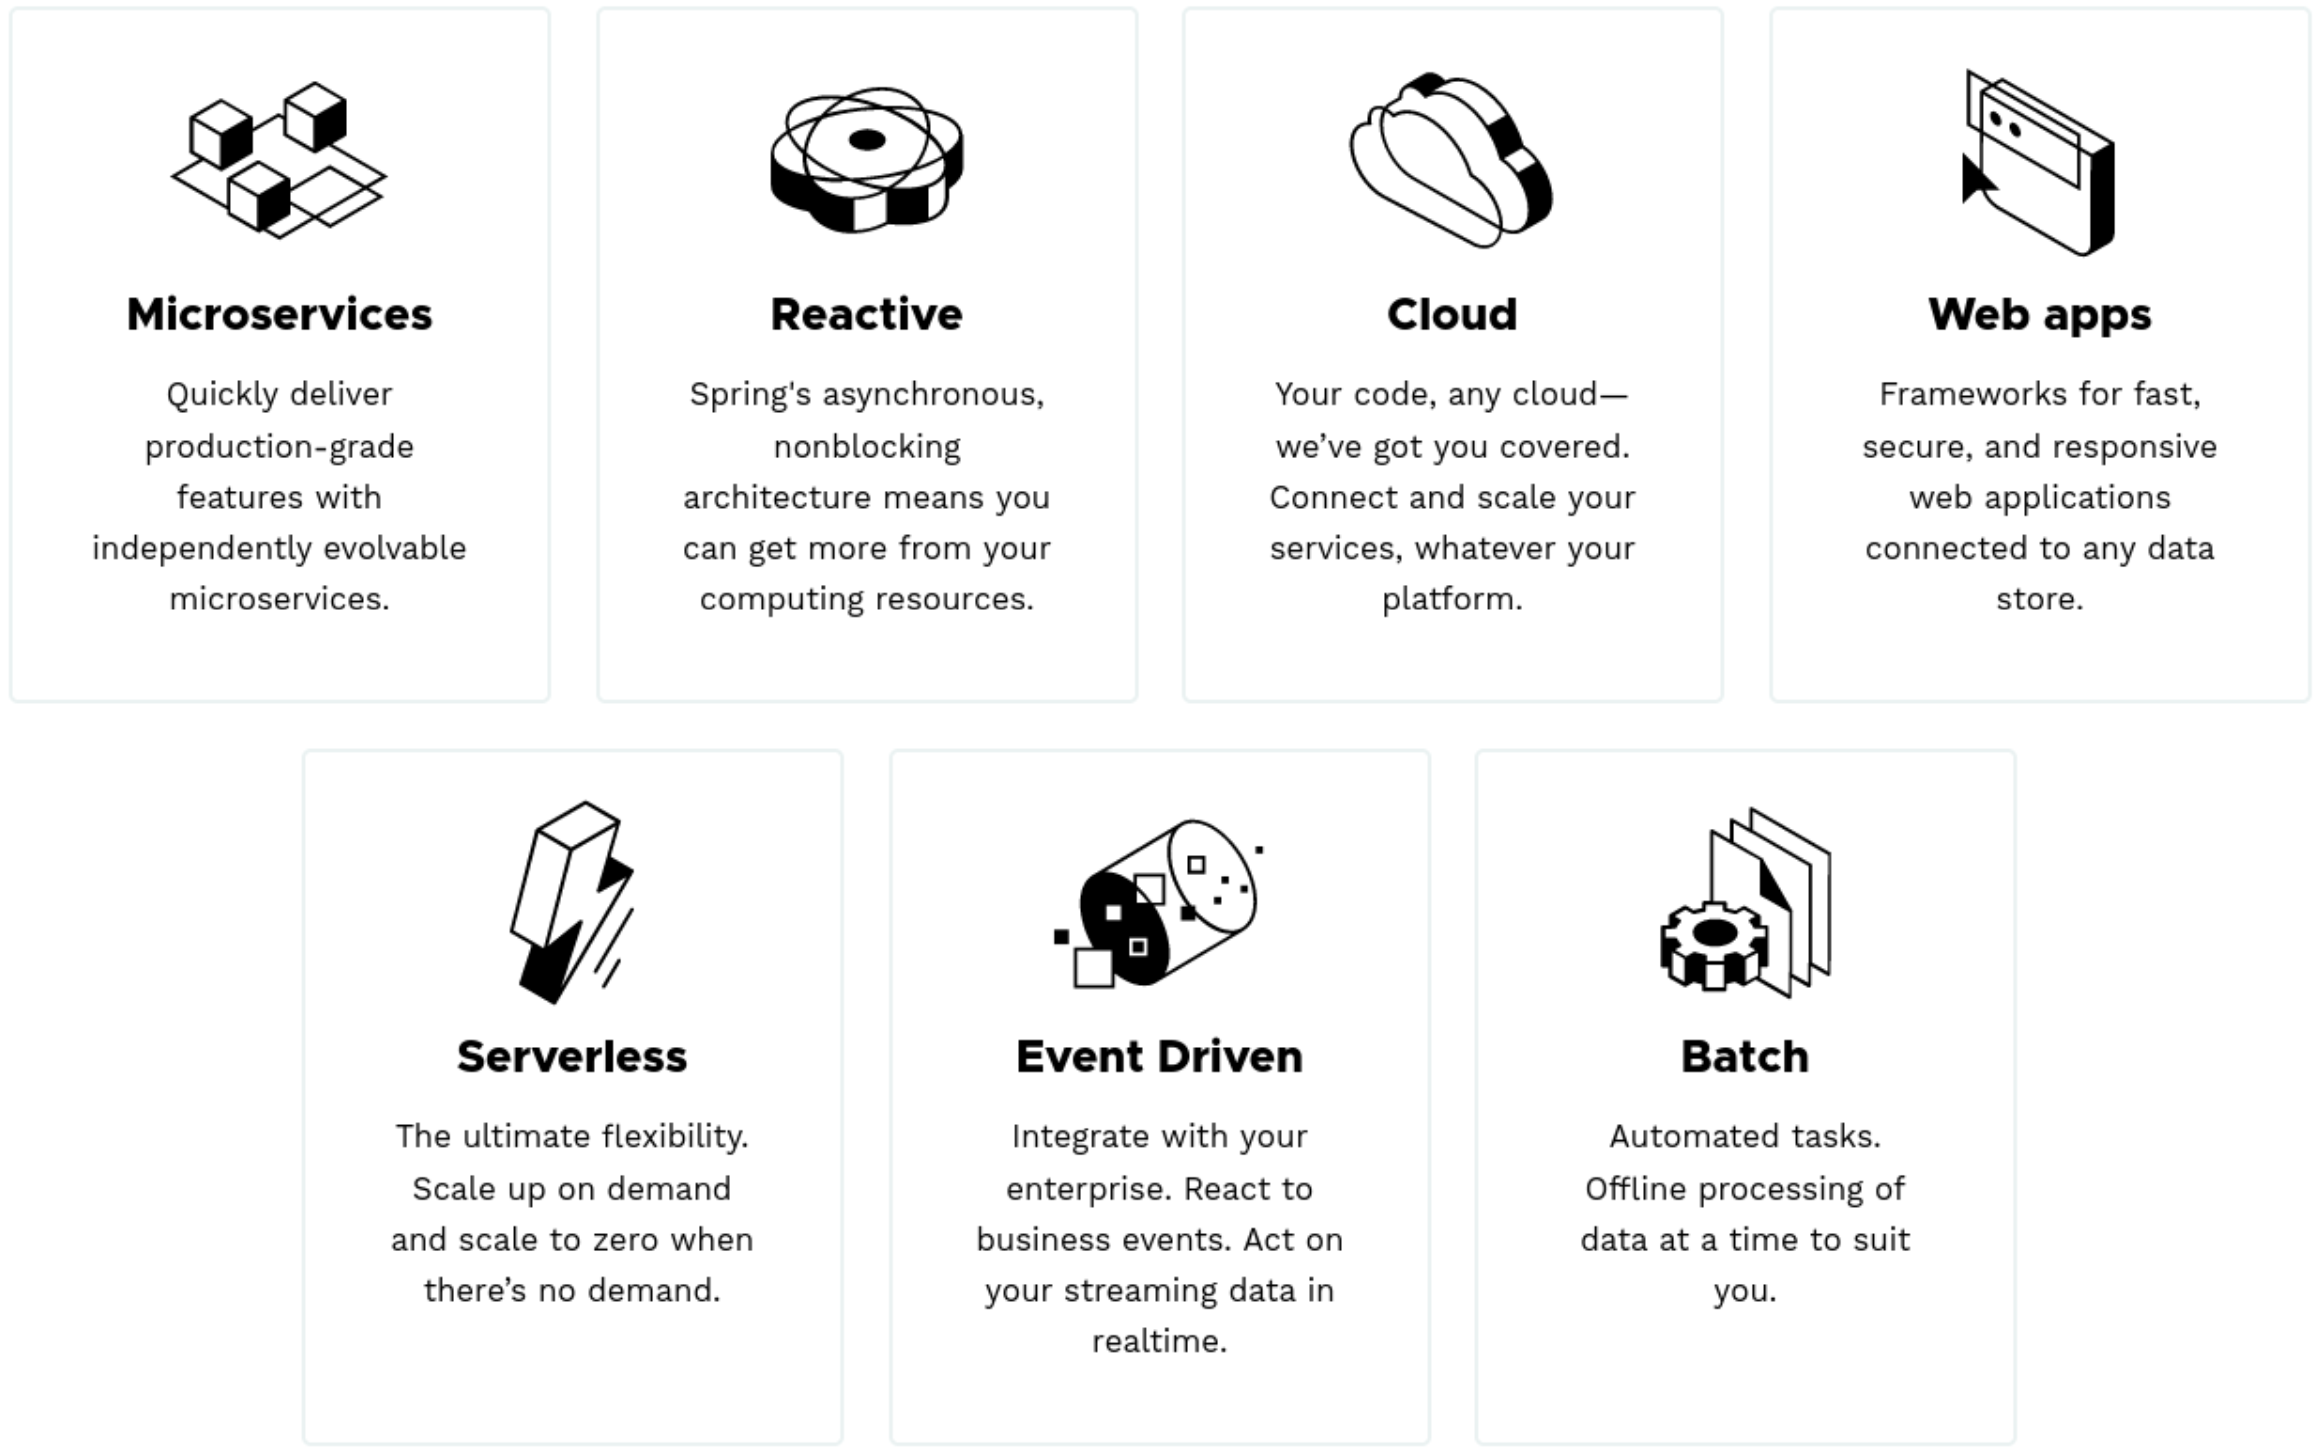
\includegraphics[width=0.75\linewidth]{images/spring.png}
    \caption{Spring framework functionalities}
\end{figure}